\documentclass{beamer}
\usetheme{Singapore}

%\usepackage{pstricks,pst-node,pst-tree}
\usepackage{amssymb,latexsym}
\usepackage{graphicx}
\usepackage{fancyvrb}
\usepackage{hyperref}

\newcommand{\bi}{\begin{itemize}}
\newcommand{\li}{\item}
\newcommand{\ei}{\end{itemize}}
\newcommand{\Show}[1]{\psshadowbox{#1}}


\newcommand{\grf}[2]{\centerline{\includegraphics[width=#1\textwidth]{#2}}}
\newcommand{\tw}{\textwidth}
\newcommand{\bc}{\begin{columns}}
\newcommand{\ec}{\end{columns}}
\newcommand{\cc}[1]{\column{#1\textwidth}}

\newcommand{\bfr}[1]{\begin{frame}[fragile]\frametitle{{ #1 }}}
\newcommand{\efr}{\end{frame}}

\newcommand{\cola}[1]{\begin{columns}\begin{column}{#1\textwidth}}
\newcommand{\colb}[1]{\end{column}\begin{column}{#1\textwidth}}
\newcommand{\colc}{\end{column}\end{columns}}


\title{Notes on Effective Learning}
\author{Based on\\
\href{http://makeitstick.net/}{\bf make it stick}\\
\em The Science of Successful Learning
\\\small Brown, Roediger \& McDaniel, 2014}

\RecustomVerbatimEnvironment{Verbatim}{Verbatim}{frame=single}

\begin{document}
\begin{frame}
\maketitle

\end{frame}



\bfr{There is no such thing as a full brain}
\begin{center}
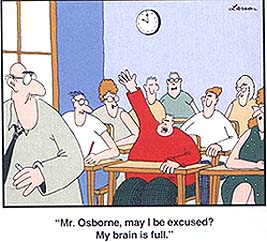
\includegraphics[height=0.7\textheight]{brainisfull.jpg}
\end{center}
\end{frame}

\bfr{There is no known limit to the capacity for learning}
\begin{description}
\li[2010] Simon Reinhard memorized 300 random words in 15 minutes.
\li[2008] Ben Pridmore memorized 884 shuffled playing cards in 30 minutes. 
\li[2010] Boris-Nikolai Konrad memorized 201 names and faces in 15 minutes.
\end{description}

\end{frame}

\bfr{Learning changes your brain}
\bi
\li Every time you learn something you {\bf change your brain}.
\bi
\li Most learning involves reinforcing connections between neurons.
\li The hippocampus, important in
long-term memory, actually creates new neurons throughout your life.
\ei
\li But these things happen in your brain {\em only if they have to.}
\li When learning is hard, you're improving your brain.
\ei
\end{frame}

\bfr{}

\setlength{\parindent}{0em}
\setlength{\parskip}{1ex}
\sl

The roughest roads often lead to the top.

\hfill --- Christina Aguilera

\end{frame}

\bfr{Learning: you're doing it wrong}
\bi
\li Learning is best when it's {\em effortful}.
\li We are {\em poor judges} of when we are learning well.
\li Bad learning habits:
\bi
\li {\em Rereading text} gives little benefit
but leads to false sense of mastery.
\li {\em Massed practiced}, repeating something over and over
until memorized, does not work.
\ei
\ei
\end{frame}

\bfr{Which penny is real?}
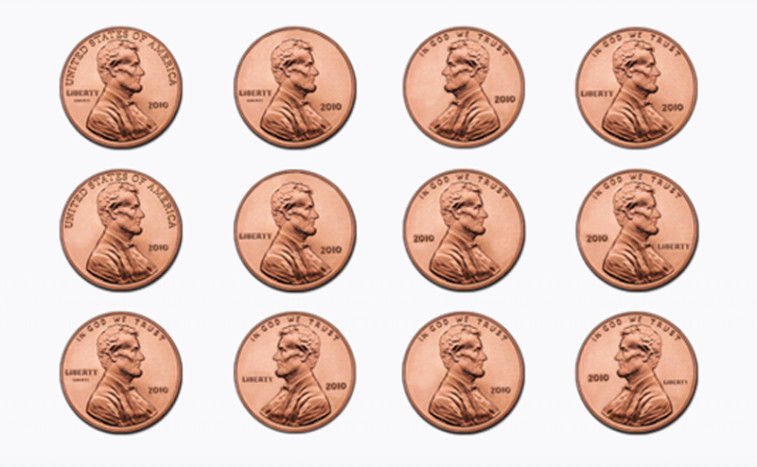
\includegraphics[width=\textwidth]{pennymemorytest.jpg}
\end{frame}

\bfr{Study {\em vs.} Testing}
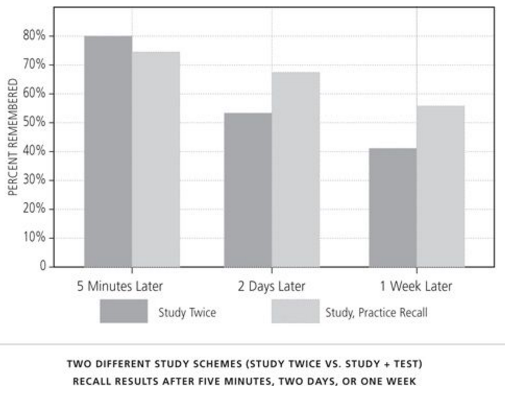
\includegraphics[width=0.9\textwidth]{studyvstest.png}
\end{frame}

\bfr{Testing {\em vs.} More Testing}
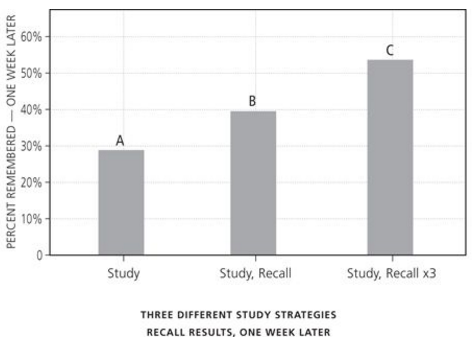
\includegraphics[width=\textwidth]{test3times.png}
\end{frame}

\bfr{Learning: doing it right}
\bi
\li {\em Retrieval practice} is far more effective.
\li Flash cards are the simplest example.
\centerline{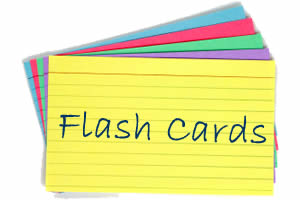
\includegraphics[scale=1.0]{flashcards.jpg}}
\li Trying to solve a problem yourself
leads to better learning,

\li ... even if you try before you know how
\li ... even if errors are made

\ei


\end{frame}

%\bfr{Learning styles:  NOT}
%\bi
%\li The popular notion that you learn better when you receive
%instruction in a form consistent with your {\em learning style}, for
%example auditory or visual, is {\bf not supported by empirical
%  evidence.} 
%\li People do have multiple learning strategies, and all people learn
%best when they ``go wide.''
%\li Limiting instruction to your preferred style reduces learning.
%\ei
%\end{frame}

%\bfr{Learning rules {\em vs.} learning facts}
%\bi
%\li When you learn underlying principles or {\bf rules} you are more
%adept at picking the right solutions in unfamiliar situations.
%\li This skill is better acquired through {\bf interleaved and varied
%  practice} than massed practice.
%\ei
%\end{frame}

\bfr{We are all susceptible to {\bf illusions} of learning}
\bi
\li Reading and rereading 
the text gives the {\bf illusion} of fluency.
\li Highlighting 
the text gives the {\bf illusion} of mastery.
\ei
\centerline{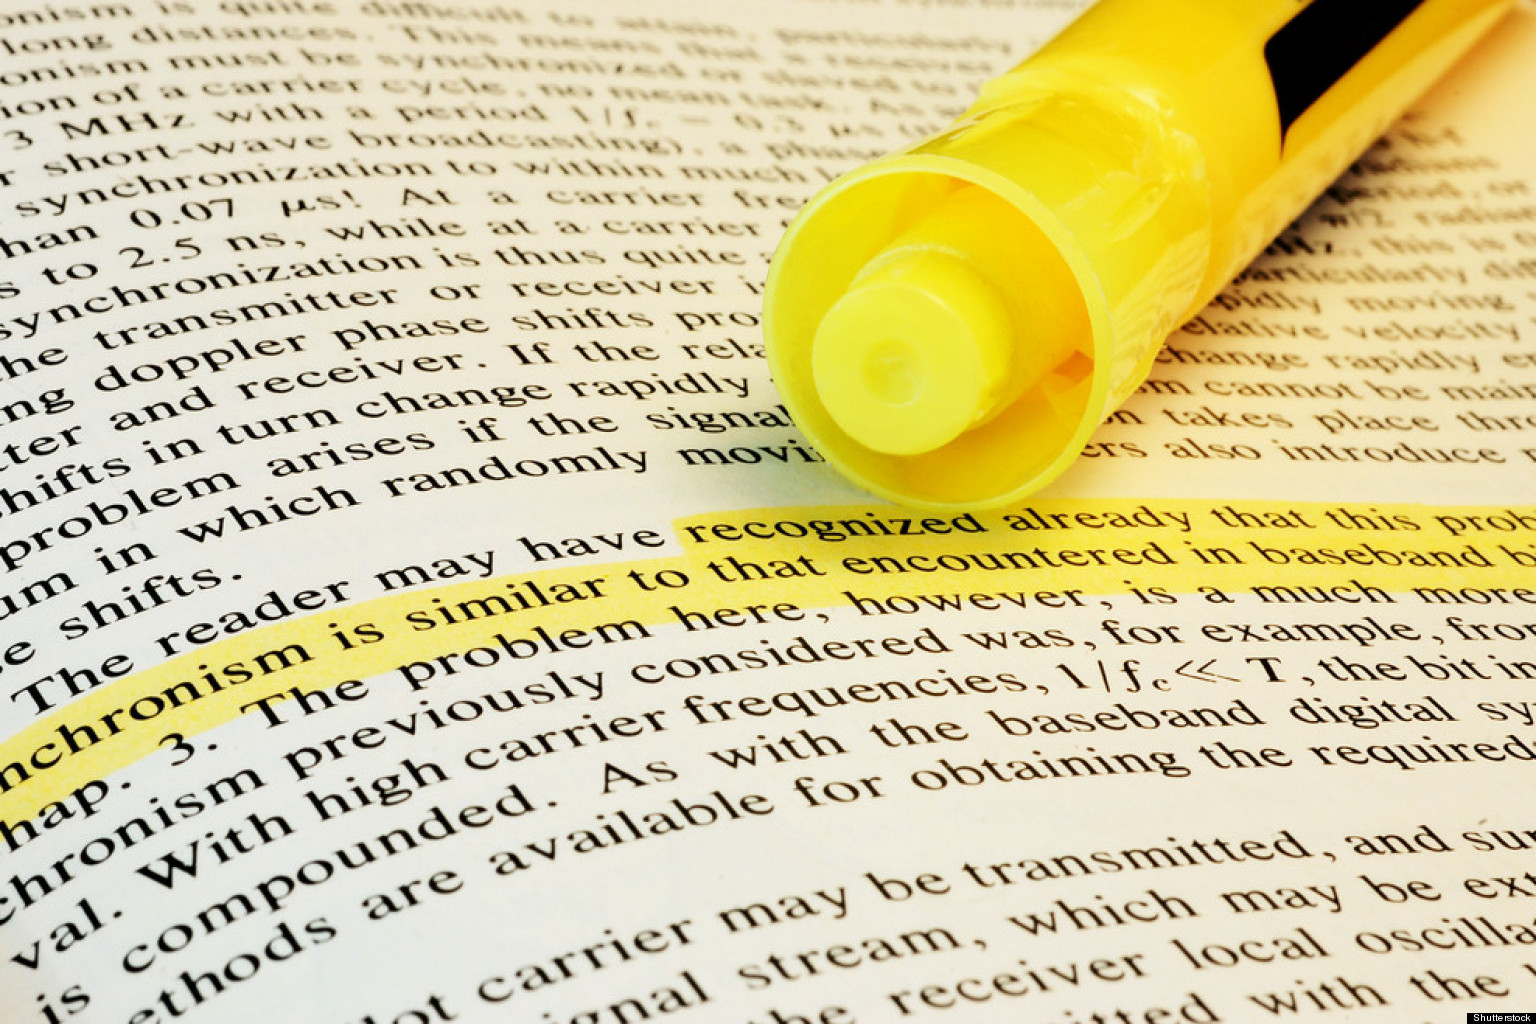
\includegraphics[width=3in]{highlighting.jpg}}
\end{frame}

\bfr{Testing dispells illusions}
\bi
\li {\bf Testing} helps calibrate our judgements.
\li Only shooting an azimuth gives us the truth.
\ei
\centerline{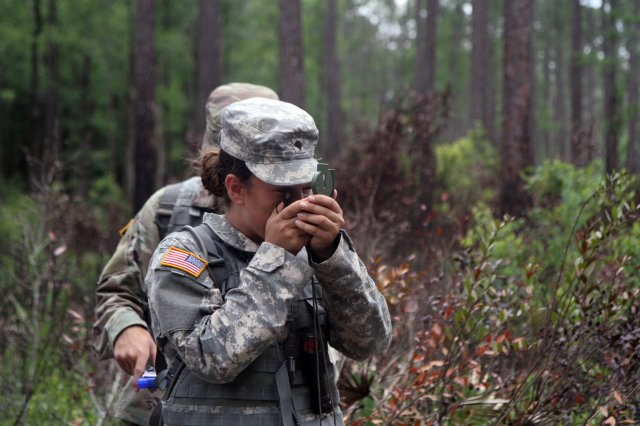
\includegraphics[width=3in]{shootinganazimuth.jpg}}
\end{frame}

\bfr{Tests: assessment {\em vs.} learning tool}


\begin{quotation}
We are what we repeatedly do. Excellence, then, is not an act, but a habit.

\hfill ---Aristotle
\end{quotation}

\vfill


 Exercise in repeatedly recalling a thing strengthens the memory.

\vfill
\end{frame}

\bfr{An experiment}
\bi
\li Subjects were given passages to read.
\li Some passages were immediately tested on.
\li Other passages were reread.
\li {\bf Tested passages were remembered better.}
\ei
\end{frame}

\bfr{Another experiment}
\bi
\li Some subjects asked to memorize pairs like {\em foot-shoe}
\li Others asked to memorize pairs like {\em foot-s\_\_e}
\li {\bf Second group did substantially better.}
\ei
\end{frame}
\bfr{}
\centerline{\huge\fbox{\sc Quizzing is a learning tool!}}
\end{frame}

\bfr{Spaced repetition is the most effective}
\begin{center}
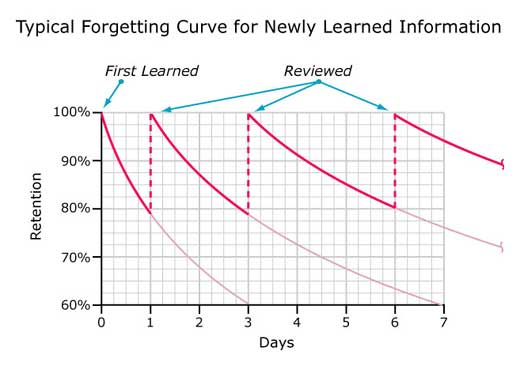
\includegraphics[width=\textwidth]{ForgettingCurve.jpg}
\end{center}
\end{frame}


\bfr{How to practice retrieving from memory}
\bi
\li Quiz, quiz, quiz!
\li Use flash cards: \url{www.ankisrs.net}
\li Use Cornell note taking system \\\url{http://lsc.cornell.edu/LSC_Resources/cornellsystem.pdf}
\li Look up from the book and summarize
\li Invent quiz questions as you read
\ei
\bi
\li Don't listen to your intuition!  Shoot an azimuth!
\li Space out retrieval practice, no cramming.
\ei
\end{frame}

\bfr{Relate it to your own experience}

\begin{description}
\item[Generation:]
  Try to answer a problem before being shown the solution.
\item[Elaboration:]
  Explain it in your own words and relate it to your own experience.
\item[Reflection:] Write out essays on your learning.
\end{description}
\end{frame}


%\bfr{}
%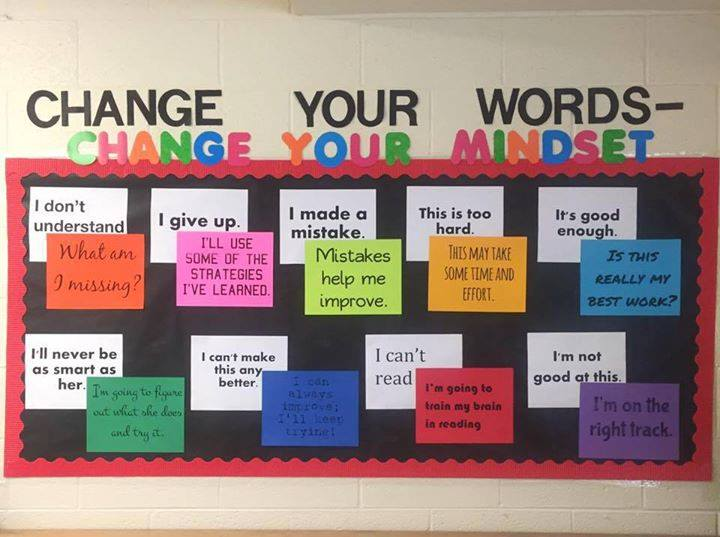
\includegraphics[width=\textwidth]{changeyourvocabulary.jpg}
%\end{frame}

\bfr{Wish for the new year}

\setlength{\parindent}{0em}
\setlength{\parskip}{1ex}
\sl




I hope that in this year to come, you make mistakes.

Because if you are making mistakes, then you are making new things, trying new things, learning, living, pushing yourself, changing yourself, changing your world. You're doing things you've never done before, and more importantly, you're Doing Something.

So that's my wish for you, and all of us, and my wish for myself. Make New Mistakes. Make glorious, amazing mistakes. Make mistakes nobody's ever made before. Don't freeze, don't stop, don't worry that it isn't good enough, or it isn't perfect, whatever it is: art, or love, or work or family or life.

Whatever it is you're scared of doing, Do it.

Make your mistakes, next year and forever.


\hfill ---Neil Gaiman
\\
\hfill creator, The Sandman

\end{frame}

\end{document}
